\chapter{Network Measurements}
\label{chp:measurements2}

This chapter will display the measured data from the accelerometer, and graphs, tables and figures to try to determine the most efficient solution. 

\section{temp/notes}

Trying to understand the details of a capture in Wireshark. 

Can fragmentation give us an advangate, if you can send more data pr header. 

An empty char array sent over CoAP is 76 bytes. 
19 bytes char array, 96 bytes
21 bytes char array, 98 bytes. Adds only as much as needed. 
 



\section{Packet fragmentation}

In Internet Routing, \textit{fragmentation} is known as the action of splitting data into smaller packets, to satisfy the maximal limits of the different technologies used (e.g. \gls{ble} and \gls{6lowpan} in the network described in this thesis). Each of these net packets needs header fields of a certain size, or other requirements.

To better understand fragmentation, imagine a train with carriages. To be able to operate at all, the train needs a locomotive with an engine driver, a conductor and a cafe carriage. As soon as these things are already there, the company owning the train gets better and better off for every passenger buying a ticket. Eventually all the carriages will be full, and a decision has to be made if it will be profitable to fit another carriage. It will in general be most profitable to use as many carriages as the locomotive can handle, and to fill up every carriage as much as possible. It will however not be a good idea to connect another carriage if there will only be one additional passenger sitting there, since the extra weight of the carriage requires additional weight to the train set. 

In this example, the locomotive and employees are the \gls{6lowpan} packet, that are needed no matter what. Each additional carriage is a \gls{ble} packet. The goal is therefore to find the maximal number of passengers compared to the cost of adding additional carriages, in other words the maximal number of bytes compared to the number of packets sent. This is known as \gls{fragmentation}, to maximize \textit{goodput} vs \textit{throughput}. 

\section{Goodput vs throughput}

When sending \gls{ble} packets over the network, observations from the system shows that the maximum packet size over \gls{ble} is 31 bytes. Each of these packages needs a header field of 4 bytes, meaning 27 bytes left for useful data. However, to start the connection at all, 76 byte is needed, meaning three \gls{ble} packets. The ratio between \textit{useful} and \textit{needed} (known as \textit{goodput} and \textit{throughput}) data transferred therefore start out very poorly if the payload sent is very small. 

\begin{figure}[ht]
    \centering
    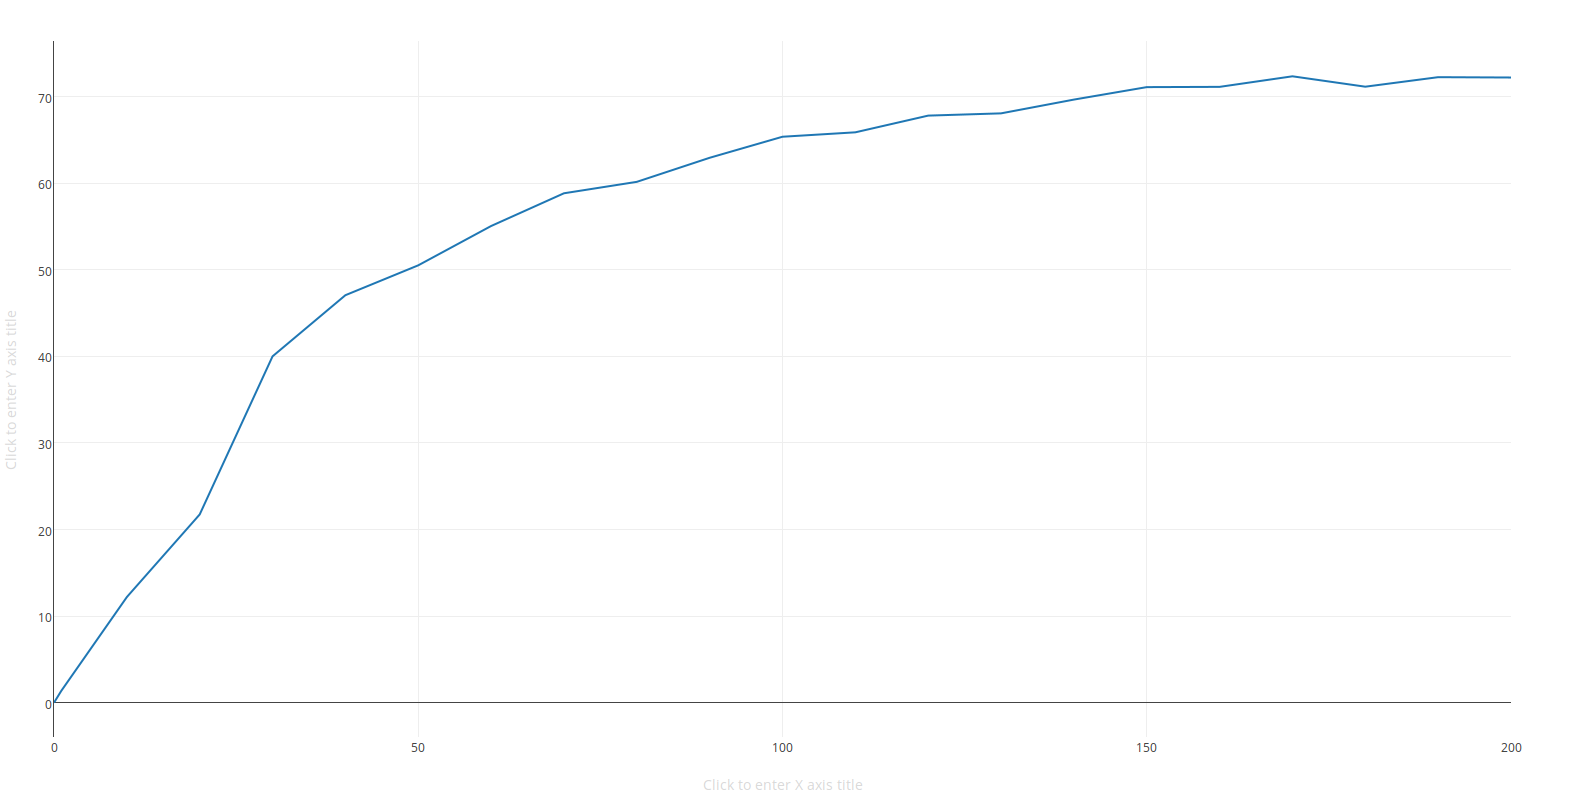
\includegraphics[scale=0.25]{graph1.png}    
    \caption{Goodput compared to throughput in \%}
    \label{fig:goodputThroughputGraph}
\end{figure}


Figure \ref{fig:goodputThroughputGraph} shows the correlation between goodput and throughput compared to the number of packets sent. In this particular case it makes no sense to send less than 50 bytes at once, since more than 50 \% of the data will be header files. But, since at least 4 bytes out of every 31 sent needs to be used to header information, the best possible result will be 87,1 \%. This graph will therefore converge to the \textit{horizontal asymptote} of 87,1 \%, just as the graph shows after just a packet size of 200 bytes. 








